\documentclass[12pt,letterpaper,final]{report}
\usepackage[utf8]{inputenc}
\usepackage{amsmath}
\usepackage{amsfonts}
\usepackage{amssymb}
\usepackage{amsthm}
\renewcommand\qedsymbol{$\blacksquare$}
\usepackage{enumerate}
\usepackage{hyperref}
\usepackage{pdfpages}
\usepackage{graphics}
\usepackage{graphicx}
\usepackage{tikz}
\usepackage{tikz-qtree}
\usetikzlibrary{automata,arrows}

\author{Marius Zimand}
\author{Jonathan Llovet}

\begin{document}

\fbox{
  \vbox{
    \begin{flushleft}
      Jonathan Llovet \\  % authors' names
      COSC 417 \\  %class
      2026-02-12, 11:59 PM (EST) \\  % date
    \end{flushleft}
    \center{\Large{\textbf{Assignment 1}}}
    %\end{mdframed}
  } % end vbox
} % end fbox
\vline

{\bf Problem 1.} Let $A = \{x,y\}$ and $B= \{x,y,z\}$.
\begin{enumerate}
  \item  Is $A$ a subset of $B$?

        Yes

  \item  Is $B$ a subset of $A$?

        No

  \item What is $A \cup B$?

        $\{x,y,z\}$

  \item  What is $A \cap B$?

        $\{x,y\}$

  \item  What is $A \times B$?

        $\{(x,x), (x,y), (x,z), (y,x), (y,y), (y,z)\}$

  \item  What is ${\cal P}(B)$? (${\cal P}(B)$ is the powerset of $B$).

        $\{
          \emptyset,
          \{x\},
          \{y\},
          \{z\},
          \{x,y\},
          \{x,z\},
          \{y,z\},
          \{x,y,z\}
          \}$

  \item What is ${\cal P}({\cal P}(A))$?

        Recall that
        \[
          \begin{array}{lll}
            A           & = \{x,y\}                              \\
            {\cal P}(A) & = \{\emptyset, \{x\}, \{y\}, \{x,y\}\} \\                                                                                                                                     \\ % quadruple
          \end{array}
        \]

        Arranging the elements by their cardinality, ${\cal P}({\cal P}(A))$ is as follows:
        \[
          \begin{array}{lll}
             & \Bigg\{ \emptyset,                                                                                                                                                               \\\\ % empty set
             & \{\emptyset\}, \{x\}, \{y\}, \{x, y\},                                                                                                                                           \\\\ % singletons
             & \Big\{\emptyset, \{x\}\Big\}, \Big\{\emptyset, \{y\}\Big\}, \Big\{\emptyset, \{x, y\}\Big\}, \Big\{\{x\}, \{y\}\Big\}, \Big\{\{x\}, \{x, y\}\Big\}, \Big\{\{y\}, \{x, y\}\Big\}, \\\\ % pairs
             & \Big\{\emptyset, \{x\}, \{y\}\Big\}, \Big\{\emptyset, \{x\}, \{x, y\}\Big\}, \Big\{\emptyset, \{y\}, \{x, y\}\Big\}, \Big\{\{x\}, \{y\}, \{x, y\}\Big\},                         \\\\ % triples
             & \Big\{\emptyset, \{x\}, \{y\}, \{x, y\}\Big\} \Bigg\}
          \end{array}
        \]

  \item What is the size of ${\cal P}(A) \times {\cal P}(B)$?


        The cardinality of a power set $X$ is $2^{\vert X \vert}$.

        $A = \{x,y\}$ and $B= \{x,y,z\}$. Their cardinalities are $\vert A \vert = 2$, $\vert B \vert = 3$.

        Hence, the size of ${\cal P}(A)$ is $2^2 = 4$, and the size of ${\cal P}(B)$ is $2^3 = 8$.

        Therefore the size of ${\cal P}(A) \times {\cal P}(B)$ is $2^{\vert A \vert} \times 2^{\vert B \vert}$, or

        $2^{2} \times 2^{3} = 4 \times 8 = 32$


\end{enumerate}

\pagebreak
{\bf Problem 2.}	Show that the set $A =\{-1, 0\} \cup \mathbb{N}$ is a countable infinite set by giving an explicit bijective function $f : {\mathbb N} \rightarrow A$.  Prove that your function $f$ is a bijection, by showing that it is 1-to-1 (no two natural numbers map to the same element) and onto (every element in $A$ is the image of some natural number).
\medskip

Let $f(n) = n - 2$.
First, we will write $A =\{-1, 0\} \cup \mathbb{N}$ as one set:

\[
  \begin{aligned}
    \mathbb{N} & = \{1,2,3,4,5,\ldots\}  \\
    A          & = \{-1,0,1,2,3,\ldots\}
  \end{aligned}
\]

By applying $f$ to each of the elements of $\mathbb{N}$ in turn, we will obtain:

\[
  \begin{aligned}
    f(\mathbb{N}) & = \{f(1), f(2), f(3), f(4), f(5), \ldots\} \\
                  & = \{-1,0,1,2,3,\ldots\}                    \\
                  & = A
  \end{aligned}
\]
We will prove that $f(n)$ is a bijection in two parts.
In the first part, we will show by contraposition that $f$ is injective, and in the second part we will show by induction that $f$ is surjective.

\medskip
{\bf Part 1: Injective (1-1)}: No two natural numbers map to the same element.

We wish to show that $f: \mathbb{N} \to A$ is injective, i.e.
\begin{equation}
  \forall a, b \in \mathbb{N}, a \ne b \implies f(a) \ne f(b) \label{eq:1}
\end{equation}

We will prove this by contraposition. The contrapositive of the preceding statement is
\begin{equation}
  \forall a, b \in \mathbb{N}, f(a) = f(b) \implies a = b \label{eq:2}
\end{equation}

This is what we will tackle to prove the original. Let
\[
  \begin{aligned}
    a & = c \\
    b & = d
  \end{aligned}
  \quad \text{where } c, d \in \mathbb{N}.
\]

Then
\[
  \begin{aligned}
     &            & f(c)  & = f(d)  &  & \text{using particular values for a, b} \\
     &            & c - 2 & = d - 2 &  & \text{by substitution for $f(n)$}       \\
     & \therefore & c     & = d     &  & \text{by adding 2 to both sides}
  \end{aligned}
\]

From preceding, we conclude \eqref{eq:2}. But therefore, because contrapositives are logically equivalent, we conclude that \eqref{eq:1} is true, viz. $\forall a, b \in \mathbb{N}, a \ne b \implies f(a) \ne f(b)$, and that the function $f$ is injective.

\medskip
{\bf Part 2: Surjective (Onto)}: Every element in A is the image of some natural number.

We wish to show that $f: \mathbb{N} \to A$ is surjective, i.e.
\begin{equation}
  \forall a \in A, \exists n \in \mathbb{N}: a = f(n) \label{eq:3}
\end{equation}

We will prove this by induction.

\medskip
{\bf Basis step: $P(A_0)$}
\medskip

We wish to show:
\begin{equation}
  \exists n \in \mathbb{N} : f(n) = A_0  \label{eq:4}
\end{equation}

Note that $A_0 = - 1$. Examining this and solving for $n$:

\[
  \begin{aligned}
    f(n)  & = -1 &  &                                \\
    n - 2 & = -1 &  & \text{by definition of $f(n)$} \\
    n     & = 1  &  & \text{by algebra}              \\
  \end{aligned}
\]

But $1 \in \mathbb{N}$. Therefore, \eqref{eq:4} holds.

\medskip
{\bf Induction step: $P(a,k) \implies P(a+1, k+1)$}
\medskip

Assume for some $a \in A$, some $k \in \mathbb{N}$ where $k \ge 1$ that
\[
  P(a,k): a = f(k)
\]

Or, more usefully, substituting for $f(k)$,

\begin{equation}
  P(a,k): a = k - 2 \tag{Inductive Hypothesis} \label{eq:5}
\end{equation}
\medskip

We wish to show that $P(a,k) \implies P(a+1, k+1)$. Consider:

\begin{align*}
  a + 1     & = f(k+1)    &  & \text{By definition of $P(a+1, k+1)$}              \\
  a + 1     & = k + 1 - 2 &  & \text{By definition of $f(k+1)$}                   \\
  k - 2 + 1 & = k + 1 - 2 &  & \text{By substitution for $a$ from $\eqref{eq:5}$} \\
  k         & = k         &  & \text{By simplification}                           \\
\end{align*}

But therefore, $P(a,k) \implies P(a+1, k+1)$ holds. Hence, we conclude by the principle of mathematical induction that \eqref{eq:3} holds. That is, we conclude that $\forall a \in A, \exists n \in \mathbb{N}: a = f(n)$, or to put it simply, that the function $f$ is surjective.

\medskip
{\bf Conclusion: $f$ is bijective, $A$ is countably infinite}
\medskip

Therefore, having shown that the function $f(n)$ is injective and surjective, we conclude that it is bijective. But therefore, by definition of a countable infinite set, we conclude further that $A =\{-1, 0\} \cup \mathbb{N}$ is a countably infinite set, since we have found a bijective function $f: \mathbb{N} \to A$.

\qed



\pagebreak
{\bf Problem 3.} For each of the following languages, give the state diagram of a DFA with the specified number of states that recognizes the language. The alphabet is $\Sigma = \{0,1\}$.

\begin{enumerate}

  \item $\{w \colon \mbox{ $w$ contains at least one $0$ and one $1$}\}$, with $4$ states.

        \medskip

        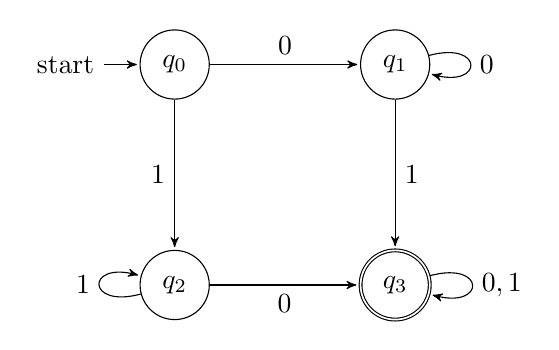
\begin{tikzpicture}[>=stealth',shorten >=1pt,auto,node distance=2.8cm]

          \node[initial, state] (0) {$q_{0}$};
          \node[state] (1) [right of=0] {$q_{1}$};
          \node[state] (2) [below of=0] {$q_{2}$};
          \node[state, accepting] (3) [below of=1] {$q_{3}$};

          \path[->]
          (0) edge node[above] {$0$} (1)
          (0) edge node[left] {$1$} (2)

          (1) edge node[right] {$1$} (3)
          (1) edge [loop right] node {$0$} (1)

          (2) edge [loop left] node {$1$} (2)
          (2) edge node[below] {$0$} (3)

          (3) edge [loop right] node {$0,1$} (3)
          ;
        \end{tikzpicture}

  \item $\{w \colon \mbox{ $w$ has $0$ in every odd position}\}$, with $3$ states.


\end{enumerate}

\pagebreak
{\bf Problem 4.}  Recall that an infinite  set $A$ is countable if there is a \emph{bijective}  function $f: {\mathbb N} \rightarrow A$.  Show that if there is an \emph{onto} function
$g: {\mathbb N} \rightarrow A$, then $A$ is countable. In other words, you need to show how you can modify $g$ to obtain a bijective function $f$ that enumerates $A$.

\pagebreak
{\bf Problem 5. }
Let $A$ and $B$  be two infinite countable sets.  Show that  $A \cup  B$ is  also an infinite countable sets. You need to show how to obtain an enumeration of $A \cup B$ if you have an enumeration $A = \{f(1), f(2), \ldots \}$ and an enumeration of $B = \{g(1), g(2), \ldots \}$ (in other words you need to explain how you can list one-by-one all the elements  in $A \cup B$.)

\end{document}
